%!TEX root = ../main.tex
%
% 原子スペクトルの観察
% レポート用紙
%

\stepcounter{section}
\section*{原子スペクトルの観察}

\begin{center}
\begin{tabular}{|c|c|c|c|}
\hline
\parbox[c][1.2cm][c]{0cm}{}学籍番号 & \hspace{3cm} & 名前 & \hspace{6cm} \\
\hline
\parbox[c][1.2cm][c]{0cm}{}実験日時 & \multicolumn{3}{|l|}{   年  月  日  曜日  時限}\\
\hline
\parbox[c][2.0cm][c]{0cm}{}共同実験者 & \multicolumn{3}{|l|}{}\\
\hline
\end{tabular}
\end{center}

\subsection*{実験の概要と目的}

%\vspace{5cm}
\newpage



\subsection*{測定値および計算}

\subjikken{簡易分光計の組み立てと原子スペクトルの観察}\\
{\bf スペクトル線のスケッチ}
\begin{center}
\hspace*{1cm}
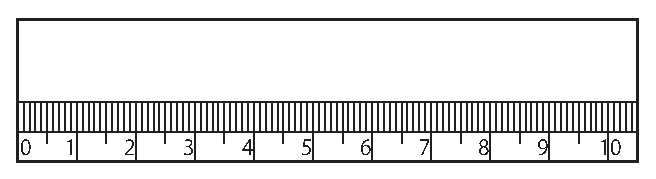
\includegraphics{12_Spectrum/scale.eps}\\
\vspace{0.5cm}
\hspace*{1cm}
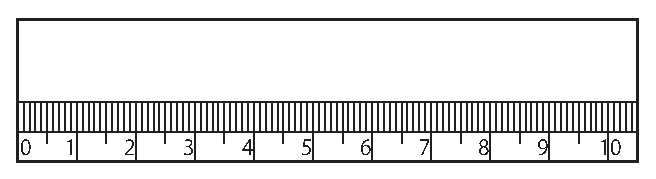
\includegraphics{12_Spectrum/scale.eps}\\
\vspace{0.5cm}
\hspace*{1cm}
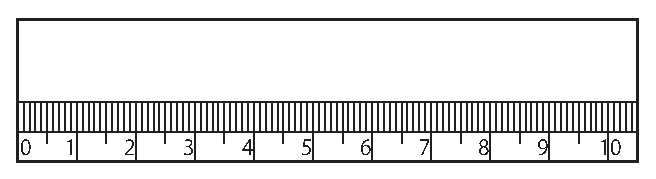
\includegraphics{12_Spectrum/scale.eps}
\end{center}

%\newpage

\subsubsection*{測定結果}
\hspace*{-\parindent}
\begin{tabular}{|c|c|c|c|c|}
\hline
No. & 色 & 位置~[cm] & 波長~[nm] & エネルギー~[eV] \\
\hline\hline
\hspace*{1.5cm}&\hspace*{2cm}&\hspace*{3.5cm}&\hspace*{3.5cm}&\hspace*{3.5cm}\\
\hline
&&&&\\
\hline
&&&&\\
\hline
&&&&\\
\hline
&&&&\\
\hline
&&&&\\
\hline
&&&&\\
\hline
&&&&\\
\hline
&&&&\\
\hline
&&&&\\
\hline
&&&&\\
\hline
&&&&\\
\hline
&&&&\\
\hline
&&&&\\
\hline
&&&&\\
\hline
\end{tabular}


\subsection*{考察}

\begin{itemize}

\item 各光源について観察した原子のスペクトルから、発光している原子の種類をそれぞれ同定しましょう。(理由を含めてきちんと考察すること。)


\vspace*{6cm}

\item 原子のスペクトルを観察することで、原子についてどのようなことがわかるでしょうか?

\vspace{6cm}

\item 原子のエネルギーを測定する単位として電子ボルト[eV]を用いる理由を考えてみましょう。
\end{itemize}
